\documentclass{statsoc}
\usepackage[a4paper]{geometry}   % otherwise statsoc class doesn't compile to A4 correctly
%\usepackage{setspace}
%\doublespacing

\usepackage[hidelinks]{hyperref} % auto detect ref type
\usepackage{natbib}
%\setcitestyle{rss}

\usepackage{graphicx}
\usepackage{amssymb}
\usepackage{amsmath}
\usepackage{enumerate}
\usepackage{caption}
\usepackage{textcomp}    % for Hawaii characters
\usepackage{url}

% to find textwidth
%\usepackage{layouts}

% new commands
\newcommand{\wt}[1]{\widetilde{#1}}
\newcommand{\ol}[1]{\overline{#1}}
\newcommand{\wh}[1]{\widehat{#1}}
\newcommand{\bbeta}{\boldsymbol{\beta}}
\newcommand{\blambda}{\boldsymbol{\lambda}}
\newcommand{\T}{\intercal}
\newcommand{\bs}{\mathbf{s}}
\newcommand{\bS}{\mathbf{S}}
\newcommand{\bQ}{\mathbf{Q}}
\newcommand{\bSigma}{\boldsymbol{\Sigma}}
\newcommand{\bm}{\boldsymbol}  % bold maths symbols
\newcommand{\tl}{\tilde{\lambda}}   % thinned little lambda
\newcommand{\tL}{\tilde{\Lambda}}  % thinned big lambda

% RJC 09/08/2019 Added shortcuts for Hawaiian words
\newcommand{\akepa}{\textquotesingle\={a}kepa}  % adds Hawaiian diacritical marks
\newcommand{\Akepa}{\textquotesingle\={A}kepa}  % adds Hawaiian diacritical marks
\newcommand{\hawaii}{Hawai\textquotesingle i}   % adds Hawaiian diacritical marks
\DeclareMathOperator*{\argmax}{arg\,max}  % * means _ puts thing beneath operator

\title[One-stage point transect distance sampling using iterated INLA]{One-stage point transect distance sampling using iterated integrated nested Laplace approximations}

\author[Andrew E. Seaton {\it et al.}]{Andrew E. Seaton}
\address{School of Biodiversity, One Health and Veterinary Medicine, 
	University of Glasgow, 
	Glasgow,
	UK}
\email{andrew.seaton.2@glasgow.ac.uk}

\author{Janine B. Illian}
\address{School of Mathematics and Statistics, University of Glasgow, Glasgow, UK}

\author{Finn Lindgren}
\address{School of Mathematics, University of Edinburgh, Edinburgh, UK}

\author{Richard J. Camp}
\address{U. S. Geological Survey, Pacific Island Ecosystems Research Center, P.O. Box 44, \hawaii{} National Park, HI 96718, U.S.A.}

% seems like this document class uses short author from the last author
% macro in the preamble?  
\author[Andrew E. Seaton \textit{et al.}]{Steve J. Kendall}
\address{U. S. Fish and Wildlife, Big Island National Wildlife Refuge Complex, 60 Nowelo St., Suite 100, Hilo, HI  96720, U.S.A.}

\begin{document}

\begin{abstract}
Distance sampling methods aim to estimate the size and spatial distribution of populations of wild animals.  In traditional analyses, spatial modelling is conducted in a second modelling stage, conditional on estimates of the detectability of animals. Here we present a one-stage analysis that simultaneously estimates the detectability and spatial distribution of an endangered tropical bird population.  We take a point process perspective, modelling animal locations as a thinned log-Gaussian Cox process.

Since the thinning process is non-linear, we cannot use standard methods for inference. To address this we use a novel approximate Bayesian inference approach based on an iterative scheme of model fits using integrated nested Laplace approximations (INLA).  This approach is general, flexible and applicable to a wide variety of non-linear model specifications. To illustrate the value of the one-stage approach we hypothesise potential model outputs that are relevant for conservation science.  Since model outputs are based on samples from the joint posterior, they naturally account for the uncertainty in the detection process, a key advantage of the one-stage model. 

\end{abstract}

\keywords{Distance sampling, Estimating abundance, Integrated nested Laplace approximation, Point processes, Spatial statistics, Species distribution modelling}

\section{Introduction}

The estimation of the abundance and spatial distribution of wild populations of animals is a critical objective in ecology and conservation \citep{schwarz_estimating_1999}.This paper presents a statistical analysis of survey data collected on a critically endangered Hawaiian forest bird, offering insights into its population size and spatial dynamics, which are crucial to guide effective conservation management decisions.  The \hawaii{} \akepa{} (hereafter \akepa{}; \textit{Loxops coccineus}; nomenclature according to \citealp{usfws_akepa_1970}) is an endemic species whose population declined dramatically during the 20th century  \citep{usfws_revised_2006, judge_akepa_2018}.  The remaining population is the focus of sustained conservation efforts and monitoring is required to inform decision-makers about changes in the overall abundance and spatial distribution through time.  

However, estimating the abundance and spatial distribution of wild populations of animals presents various statistical challenges. Traditional methods are usually split into two stages, where the spatial distribution is estimated in a second-stage spatial model, conditional on estimates of the probability of detecting animals given they are present.  This detectability is estimated in a first-stage distance sampling model \citep{millerExtendingDensitySurface2021, miller_spatial_2013}.  The two-stage approach requires either the loss of uncertainty from the first stage, or the use of approximate methods to propagate uncertainty between the modelling stages \citep{bravington_VariancePropagationDensity_2021}.  In this paper, we present the first one-stage analysis of point transect distance sampling data that simultaneously estimates the non-linear detectability and spatial distribution of the \akepa{} population.  In order to achieve this, we take a point process perspective on distance sampling survey data which requires the use of a novel approach to inference that allows estimation of non-linear parametric model components within a generalized additive model framework. This approach is based on an iterative scheme of successive fits using integrated nested Laplace approximations (INLA) \citep{rue_approximate_2009} that is implemented in the software package \texttt{inlabru} \citep{lindgren_inlabru_2024}.  This approach is flexible, general and applicable in a wide range of contexts beyond modelling species distributions.

Since the existing \akepa{} population numbers in the thousands and lives in dense tropical forest, logistical and ecological challenges mean a full census of the population is not feasible. The \hawaii Forest Bird Survey (HFBS) \citep{scott_HFBS_1986} is a large-scale, quantitative survey of Hawaiian forest birds.  Annual surveys of the \akepa{} study-region consist of a number of point transects located at approximately regular intervals along randomly located line transects.  At these surveyed locations, the detectability of animals is unknown and must be estimated in order to convert observed counts into estimates of the total population size.  The \akepa{} survey estimates detectability using a point transect distance sampling approach \citep{buckland_distance_2015} where, for each observation, the distance to the observer is recorded. 

Additionally, a key aim of the analysis is to predict animal density at unsurveyed locations.  If animal density is modelled using spatial covariates then the covariate effects estimated in the surveyed region can be extrapolated to unsurveyed locations.  However, in many ecological contexts there is good reason to believe there are drivers of the spatial distribution for which we have no suitable explanatory covariates available. For the \akepa{} data, there is a clear example of an unexplained driver of the spatial distribution where the population favours the southern region of the preserve.  No straightforward explanatory cause has been found for this preference \citep{camp_dsm_2020}.  From a statistical perspective, we address this unexplained heterogeneity by including a spatially structured random effect in the model.  

These challenges in analysing distance sampling survey data mean that the resulting statistical model is necessarily complex. Since the \akepa{} data are collected with the clear objective of monitoring the population and informing conservation management decisions, there is a challenge for statisticians to effectively communicate with stakeholders who have a wide range of statistical expertise. We believe the Bayesian one-stage approach is a useful step to support statisticians in this task.  Since model outputs are based on Monte Carlo samples from the joint posterior, summary outputs naturally marginalise over the uncertainty in the observation process in a way that would be challenging in the traditional maximum-likelihood two-stage context.  We discuss various challenges associated with communicating uncertainty in mapped estimates of animal density and propose some illustrative alternatives that make use of the Bayesian one-stage perspective.

The paper is structured as follows:  Section \ref{sec-study-design} describes the \akepa{} study region and survey design; Section \ref{sec-ds-pp} reviews current approaches to distance sampling and presents the point process perspective; Sections \ref{sec-iinla} describes the iterated INLA fitting procedure and the spatially-structured random effect; and Sections \ref{sec-results} presents results of the analysis, model evaluation and effective communication of uncertainty.  Section \ref{sec-discussion} discusses potential extensions of the model and wider uses for iterative INLA.

\section{\Akepa{} survey design}
\label{sec-study-design}

The \hawaii{} \akepa{} is an internationally and federally endangered Hawaiian honeycreeper (\citealp{usfws_akepa_1970, birdlife_akepa_2016}) that is endemic to the island of \hawaii{}, USA.  Large-scale, quantitative surveys of Hawaiian forest birds and their habitat commenced in the mid-1970s through the HFBS \citep{scott_HFBS_1986}. Information from the HFBS is used to update the International Union for Conservation of Nature redlist \citep{iucn_redlist_2022}, where the \akepa{} is currently listed as endangered. HFBS data is also used to establish preserves that coincide with native bird hotspots, including Hakalau Forest Unit of the Big Island National Wildlife Refuge Complex on the island of \hawaii{} (hereafter Hakalau).  Hakalau is the first wildlife refuge established in \hawaii{} with the primary purpose to protect and manage native forests for the conservation of threatened and endangered bird and plant species.

During the 20th century, the \akepa{} population declined dramatically due to habitat modification \citep{scott_HFBS_1986, pratt_avifaunal_1994},  mosquito-transmitted avian diseases \citep{pratt_avifaunal_1994, atkinson_wildlife_1995}, introduced predators \citep{lepson_akepa_1997}, and food resources competitors \citep{lepson_akepa_1997}. \Akepa{} has a global abundance of approximately 16,200 (95\%CI 10,000\textendash25,200) birds that is now restricted to five spatially distinct populations \citep{judge_akepa_2018}. Hakalau supports the largest remaining distinct \akepa{} population which, in 2012, was estimated at more than 11,000 birds \citep{camp_statespace_2016}. Maintaining and expanding the \akepa{} population at Hakalau is a primary conservation concern. Unbiased and precise abundance estimates are required by land and resource managers for the purposes of evaluating management actions and developing future management plans.

\subsection{Point transect surveys}

Hakalau was established in 1985 to conserve 15,390 ha of montane forest habitat for native forest birds and rainforest plants. Annual forest bird surveys were initiated in 1987 to determine the population status and track trends in abundance. Survey points were established along 14 line transects following a systematic, random design with point transects located approximately 150m apart on line transects located either 500m or 1,000m apart. We limit our study area to the open-forest and closed-forest strata of Hakalau (\autoref{fig:2002studyareapointspt}), an extension of the area considered in \cite{camp_population_2010, camp_statespace_2016}, who omitted the closed-forest stratum because it was not sampled in the early years of the surveys.  For our analysis, we use data from a later year in which the closed-forest stratum was sampled and so broaden the extent of spatial inference compared to previous studies.  The open-forest stratum was previously heavily grazed, and, since the removal of cattle in 1988, regeneration has proceeded naturally \citep{maxfield_hakalau_1998}. The closed-forest stratum was historically least modified by grazing and is relatively intact forest habitat.  The northern boundary of the study area follows the refuge boundary while to the east it is bounded by a fence line (Fig. \ref{fig:2002studyareapointspt}). The southern boundary is the same as that in \cite{camp_population_2010}, chosen to exclude unsurveyed regions to the south of Hakalau but does not represent a physical boundary. To the west of the study area is pasture that is dominated by grass and is unsuitable habitat for \akepa{} and the boundary here marks the edge of the forest.

\begin{figure}[!htb]
	\centering
	\includegraphics{figures/study_area_design.pdf}
	\caption{Study area showing the 2002 survey points (black dots) in Hakalau Forest Unit of the Big Island National Wildlife Refuge Complex on the island of \hawaii{}.  The red outline marks the study area boundary as defined in \cite{camp_dsm_2020}.}
	\label{fig:2002studyareapointspt}
\end{figure}

The survey follows a point transect distance sampling design, recording the horizontal distances from observers to detected birds. Surveys commenced at dawn and continued until 11:00 or halted when weather conditions exceeded prescribed conditions that hindered detecting birds (light rain, and wind and gust strength greater than Beaufort scale 3). During 8-minute counts, trained observers recorded the species, distance to the nearest metre for each bird detected. \cite{camp_population_2010,camp_statespace_2016} provide a detailed description of Hakalau, the study area and the bird surveys.

To demonstrate our approach we selected a single survey year from the \akepa{} time series that contains a broad sampling of the study area with sufficient numbers of detections to estimate detectability. In 2002, there were a total of 289 point transects sampled within the 4,603 ha study area of Hakalau (Fig. \ref{fig:2002studyareapointspt}).  A total of 276 \akepa{} was detected on 121 point transects. The number of detections within each point transect ranged from zero to six. We selected data from a single year to demonstrate our approach in a simplified setting that does not require a temporal model component.  The choice of year is somewhat arbitrary and our model has also been applied to data from other years with similar results to those presented here.  Our approach is readily extendible to a multi-year analysis, similar to that in \cite{camp_dsm_2020}, which we discuss in more detail in Section \ref{sec-discussion}.

\section{Distance sampling as a thinned point process}
\label{sec-ds-pp}

\subsection{Overview of distance sampling methods}

Distance sampling methods aim to estimate abundance by using a spatially explicit sampling design and a parametric detection function to estimate the detectability of animals as a function of distance from transect or observer \citep{buckland_distance_2015}.  Standard distance sampling approaches use a hybrid of design- and model-based inference to estimate population size.  The probability of detection is modelled using a parametric function and, given estimates of detectability, a randomized sampling design allows for the construction of Horvitz-Thompson-like estimators of animal density \citep{ buckland_advanced_2004, horvitz_generalization_1952}.  Under this approach, animal density is uniform within each strata of the survey.  

More recently, interest has focused on fully model-based approaches that model a spatially varying animal density and allow for the use of non-random survey designs.  These methods allow animal density to be associated with spatially-indexed covariates and non-parametric random effects.  Under the model-based paradigm, animal density can, in principle, be estimated or predicted for any subregion within the study area \citep{buckland_model-based_2016, miller_spatial_2013, johnson_model-based_2010} and spatially-varying density estimates are not restricted by the stratification design that is required for Horvitz-Thompson-like estimators.  This additional flexibility allows for predictions at user-specified geographic units, such as sub-regions of nature reserves, and also for extrapolating covariate relationships to unsurveyed regions.  These features have made the model-based distance sampling paradigm a common approach in the literature \citep{garciabaron_modelling_2019, herr_aerial_2019, breen_new_2017, williams_chilean_2011, stokes_monitoring_2010, williams_modeling_2006}.

Model-based distance sampling has most commonly been implemented in a two-stage modelling framework.  In the first stage, detectability is estimated using binned counts of observed distances to fit a detection function.  In the second stage, detectability estimates from the first stage are used as an offset term in a generalized additive model framework.  Detections are are also binned into counts within user-defined sampling units (point transects or segments of line transects) and an appropriate response distribution is chosen to model these counts.  The \texttt{dsm} package \citep{miller_spatial_2013}, for example, provides tools to do this using the \texttt{R} package \texttt{mgcv} \citep{wood_gam_2017} to implement the spatially-explicit count model.  This two-stage model is known as a \textit{density surface model} and \cite{miller_spatial_2013} provide a review.

A key concern with the two-stage approach is the propagation of uncertainty from the detection model to the spatial model.  Early attempts to address this focused on bootstrapping \citep{hedley_spatial_2004, lahiri_resampling_2003}.  More recently, the bootstrap approach has been brought into question due to the difficulty of choosing the resampling units when combining spatially structured random effects and spatial bootstraps \citep{bravington_VariancePropagationDensity_2021, williams_chilean_2011}. Instead, \cite{bravington_VariancePropagationDensity_2021} propose avoiding bootstrapping completely by propagating error based on a second-order Taylor approximation of the detection function at the first-stage maximum-likelihood estimate.

Concerns about uncertainty propagation can be avoided by using one-stage modelling approaches.  A popular one-stage maximum-likelihood method, introduced by \cite{royle_ModelingAbundanceEffects_2004} and implemented in the \texttt{R} package \texttt{unmarked} \citep{fiske_UnmarkedPackageFitting_2011}, is based on reformulating the model as a multinomial likelihood.  This depends on choosing discrete distance classes and binning the data into counts defined on discrete spatial units.  Given these discrete units, the likelihood can be written in a multinomial form and, by marginalising out site specific abundance, the authors derive a Poisson likelihood to which standard maximum-likelihood methods can be applied. This approach rests heavily on the discretisation of both the distance data and the spatial location data. 

Our approach, which we outline below, is to instead adopt a point process perspective that does not require a discretisation step in either the distance or spatial location data. Although discretisation is required, it occurs at the level of a latent Gaussian random field, i.e. the model predictor vector, and not at the level of binning observations. 

In contrast to the maximum likelihood approach, Bayesian one-stage approaches have tended to use data augmentation to model unobserved individuals or groups \citep{schmidt_using_2012}, with inference via Markov chain Monte Carlo (MCMC) methods.  \citet{oedekoven_bayesian_2014} present a one-stage model that avoids data augmentation by specifying a combined likelihood of the detection and spatially-explicit count models and incorporated model uncertainty using reversible jump MCMC.

The only Bayesian one-stage analysis that does not use MCMC is, to the best of our knowledge, \citet{yuan_point_2017}, who use INLA and present an application to line transect distance sampling data.  \citet{yuan_point_2017} also take a point process perspective and formulate the detection model as a thinning of a point pattern.  Key to their approach is formulating the detection model as the solution to an stochastic partial differential equation (SPDE), a formulation that is unfamiliar to most distance sampling practitioners.

A downside to this approach is that the solutions to the detection model SPDE are not necessarily monotonically decreasing, which is a critical assumption of detection functions \citep{buckland_distance_2015}. The authors' suggestion to reject any non-monotonically decreasing functions when sampling from the posterior is potentially computationally wasteful. These differences with traditional distance sampling methods have perhaps lead to low uptake amongst practitioners of this approach, despite the computational advantages of INLA for spatial modelling. Here, we present an approach that is inspired by \citet{yuan_point_2017} but with some key differences. We also fit the model using INLA and take advantage of the benefits of the increased computational efficiency compared to MCMC.  However, we use a well-known parametric family of detection functions, that is familiar to users of classical distance sampling methods. This results in components of the model predictor that are non-linear in their parameters, making model fitting infeasible using standard INLA methods \citep{rue_approximate_2009}.  We address this by using a novel method of iterated model fits based on a first-order Taylor expansion of the non-linear model components.  Our approach is implemented in the \texttt{inlabru} package \citep{lindgren_inlabru_2024, bachl_inlabru_2019}, which also has support for spatial data objects.

Our analysis is, to the best of our knowledge, the first analysis of point transect distance sampling data formulated as a realisation of a thinned point process.  This requires a slightly more involved derivation of the relevant intensity functions compared to the line transect case in \cite{yuan_point_2017}. However, the point process perspective on distance sampling is not new and has been applied numerous times in analyses of line transect data \citep{buckland_model-based_2016, niemi_bayesian_2010, johnson_model-based_2010, waagepetersen_likelihood-based_2006, hedley_spatial_2004,  hogmander_random_1991, stoyan_remark_1982}.

\subsection{The point process model}

This section describes the statistical model for the spatial pattern of observed animal locations and distances to observers. We assume the location of all animals, detected or not, form a point pattern distributed as a log-Gaussian Cox process with intensity process $\lambda(\bs)$.  The log-Gaussian Cox process is a flexible model that can include spatial covariates to model the mean intensity as well a mean-zero spatially structured random effect to account for unexplained heterogeneity not captured by the covariates \citep{moller_log_1998}.  To account for the imperfect detection of points we specify a thinning probability function $g(\bs) = \mathbb{P}(\text{a point at $\bs$ is detected } |\text{ a point is at $\bs$})$. A key property of the log-Gaussian Cox process is that the point pattern of \textit{detected} points itself follows a log-Gaussian Cox process with intensity process $\tl(\bs) := \lambda(\bs)g(\bs)$.  Using a log link $\log g(\bs)$ is therefore included in the model as an additive component to the model for $\log \lambda(\bs)$.  

Distance sampling models specify the thinning function $g(\bs)$ as a function that decays as distance increases.  The type of distance measured depends on the type of survey.  For line transects the perpendicular distance to the transect line is used whereas for point transects it is the horizontal distance to the observer.  For the remainder of the paper we assume a point transect survey design and hence horizontal distance to an observer located at the centre of each point transect.  The thinning probability function is specified as a parametric family of functions. We denote the distance of a point at $\bs$ from an observer as $r(\bs)$.  The \textit{half-normal} detection function is $g(\bs | \sigma) = \exp(-r(\bs)^2 / 2\sigma^2)$, where $\sigma^2 > 0$ is a variance parameter to be estimated.  Other types of detection function, such as hazard-rate, negative exponential, can also be used. Their parameters themselves can be modelled using appropriate link functions to incorporate covariates that may affect detectability.  In addition to these parametric forms, additional adjustments have been proposed to increase the flexibility of such models by including trigonometric series expansions \citep{buckland_distance_2015}.  For simplicity, $\sigma$ is modelled using only an intercept parameter, but our approach can readily be extended to include covariates.

The detection function parameters can only be estimated if a uniformity assumption is made about the distribution of animals with respect to $r(\bs)$. Without such an assumption, the detection probability and intensity are confounded.  The standard assumption in distance sampling is that the intensity is constant with respect to changes in $r(\bs)$. The usual approach for two stage models is to assume $\lambda(\bs)$ is constant within each spatial unit.  With the point process perspective we are able to relax this assumption slightly to allow $\lambda(\bs)$ to be a linear function within each transect.

To describe the model in general we assume a point transect distance sampling survey consists of a set of $K$ point transects.   We denote $k$-th point transect as $\Omega_k \subset \mathbb{R}^2$ and the total surveyed region is $\Omega = \cup_{k=1}^K \Omega_k$.  In the HFBS the point transects are non-overlapping disks all with equal radius $W$ and centres at locations $\bs_k$ for $k = 1, \ldots, K$.  The probability of observing a point at location $\bs \in \Omega_k$, given there is a point at that location, we denote by $g_k(\bs)$.  The probability of observing a point outside the surveyed region is zero.
Since the point transects are non-overlapping, each location $\bs \in \Omega$ is unambiguously associated with a single observer and, therefore, a single thinning probability function $g_k$.   The half-normal detection function for points in $\Omega_k$ is therefore $g_k(\bs) = \exp(-\lVert \bs - \bs_k \rVert_2^2 / 2\sigma^2)$.  The assumption of non-overlapping survey regions could be relaxed by including extra information such as the time of each observation and observer indentifiers.  The thinning probability function for any $\bs \in \Omega$ is then given by $g(\bs) = g_{k(\bs)}(\bs)$ where $k(\bs)$ is an indexing function such that $k(\bs) = k$ whenever $\bs \in \Omega_k$.

The thinned log-Gaussian Cox process likelihood for observed points at locations $\bm{Y} = (s_1, \ldots, s_n)^\intercal$ is
\begin{equation}
\label{lgcp-likelihood}
\pi(\bm{Y}) = \exp\left( |\Omega| -\int\displaylimits_{\bs \in \Omega} \lambda(\bs) g(\bs) \mathrm{d}\bs \right)\prod_{i=1}^n \lambda(\bs_i)g(\bs_i),
\end{equation}
where $|\Omega|$ is the area of the total surveyed region and $\lambda(\bs)$ and $g(\bs)$ both depend on parameter vectors omitted for readability.  

\subsection{The modified Poisson likelihood}
\label{sec-lgcp}

\sloppy The likelihood \eqref{lgcp-likelihood} contains an integral that cannot be solved analytically.  A common approach for fitting log-Gaussian Cox processes in practice is to approximate the likelihood by replacing the integral with a weighted sum.  In this section we describe this approximate likelihood and show how it can be written as a modified Poisson likelihood which allows us to use INLA for inference.  We adapt the approach given in \cite{simpson_going_2016} for a fully observed log-Gaussian Cox process, modified to account for the point transect distance sampling observation process.

To evaluate the integral we use polar coordinates notation $\bs_k(r, \theta) = \bs_k + r\left[\cos\theta, \sin\theta \right]^T$ with $r \in [0, W]$ and $\theta \in [0, 2\pi]$ to represent locations in each sampling unit $\Omega_k$.  In a slight abuse of notation, $\bs_k$ denotes the centre of the point transect and $\bs_k(r,\theta)$ describes a location within the $k$-th point transect. The thinning function $g_k(\bs_k(r, \theta))$ depends only on $r$ and not on $\theta$ and so we use the shorthand notation $ g(\bs_k(r, \theta)) = g_k(r)$. The integral in the likelihood can be simplified using an assumption that $\lambda(\bs)$ is linear within each sampling unit.  This implies that $\lambda(\bs_k(r, \theta)) + \lambda(\bs_k(r, \theta + \pi)) = 2\lambda(\bs_k)$.  Therefore
\begin{align}
\label{eq-linear-intensity}
	\int_0^{2\pi} \lambda(\bs_k(r, \theta))g_k(r)\mathrm{d}\theta &= \int_0^\pi \{\lambda(\bs_k(r, \theta)) + \lambda(\bs_k(r, \theta + \pi) \} g_k(r)\mathrm{d}\theta \nonumber \\
	&= 2\pi \lambda(\bs_k)g_k(r).
\end{align}
We note that this is a relaxation of the traditional assumption in distance sampling that the intensity is constant within each sampling unit.  A similar relaxation is also possible in the case of line transects \citep{yuan_point_2017} and this assumption complements the choice of piecewise linear basis functions used for the spatially-structured random effect described in Section \ref{sec-gmrf}.  

It follows that $\int \lambda(\bs)g(\bs) \mathrm{d}\bs = \sum_{k=1}^K 2\pi \lambda(\bs_k) \int_0^W r g_k(r)\mathrm{d}r$ by applying the change of variables formula for integration and substituting in \eqref{eq-linear-intensity}.  This integral now only involves the one-dimensional integral with respect to $r$, greatly simplifying the integration required to evaluate the likelihood.  For each sampling unit we approximate this integral using a midpoint integration method with $M$ integration locations $r_{k1}, \ldots, r_{kM}$ and associated weights $\alpha_{k1}, \ldots, \alpha_{kM}$.  This gives
\begin{equation*}
	\int\displaylimits_{\bs \in \Omega} \lambda(\bs)g(\bs)\mathrm{d}\bs \approx \sum_{k=1}^K \sum_{j=1}^M \tilde{\alpha}_{kj} \tl(\bs_{kj}) ,
\end{equation*}
where $\tilde{\alpha}_{kj} = 2\pi \alpha_{kj}r_{kj}$ and $\tl(\bs_{kj}) = \lambda(\bs_k) g_k(r_{kj})$.

To simplify notation below we gather all integration weights into the vectors $\tilde{\alpha}_{k} = (\alpha_{k1}, \ldots, \alpha_{kM})^\intercal$ and $\tilde{\alpha} = (\alpha_1^\intercal, \ldots, \alpha_K^\intercal)^\intercal$.  Similarly, let $\tl_k = (\tl(\bs_{k1}), \ldots, \tl(\bs_{kM}))^\intercal$, $\tl_{int} = (\tl_1^\intercal, \ldots, \tl_K^\intercal)^\intercal$, the thinned intensity evaluated at each integration location, and $\tl_{obs} = (\tl(\bs_1), \ldots, \tl(\bs_n))^\intercal$, the thinned intensity evaluated at each observation location.  Then the approximate log-likelihood can be written as
\begin{equation}
\label{approx-log-likelihood}
	\log \pi(\bm{Y}) \approx - \tilde{\alpha}^\intercal \tl_{int} + 1^\intercal\log\tl_{obs}.
\end{equation}
This approximate likelihood can be expressed as a modified Poisson likelihood by letting $\eta = (\tl_{int}^\intercal, \tl_{obs}^\intercal)^\intercal$,
$\alpha = (\tilde{\alpha}^\intercal, 0_{n \times 1}^\intercal)^\intercal$ and constructing a vector of pseudo-observations $z = (0_{KM\times 1}^\intercal, 1_{n \times 1}^\intercal)^\intercal$.  Then the approximate likelihood is
\begin{equation}
\pi(\bm{Y}) \approx C \prod\limits_{i=1}^{KM + n} \eta_i^{z_i}\exp(-\alpha_i\eta_i),
\end{equation}
where $C$ is a constant.  This approximate likelihood is implemented in \texttt{inlabru} as a \texttt{"cp"} likelihood.  

The approach taken here is similar to the Berman-Turner device \citep{baddeley_practical_2000, berman_approximating_1992} that is used to fit a wide variety of point process models using GLM software.  The main difference with our approach is that we do not use the assumption that the locations of observed points form a part of the quadrature scheme.

\subsection{Intensity functions for incomplete data}

In the above, we assume the data are complete records of animal locations.  That is, each observation has a known position $\bm{y}_i = \bs_{k(\bs_i)}(r_i, \theta_i)$.  However, in many distance sampling surveys only the location of the observer and the distance to the observer are recorded.  Data of this type can be analysed within a point process framework by deriving the appropriate intensity function for this censored data. If only $r$ is recorded and $\theta$ is unknown, the intensity for points at a distance $r$ observed within point transect $\Omega_k$ is
\begin{align}
\label{intensity-incomplete}
\tl_k(r) &= \oint\displaylimits_{c_k(r)} \lambda(\bs)g_k(r)\mathrm{d}\bs \nonumber \\
&= 2\pi\lambda(\bs_k)rg_k(r),
\end{align}
where $c_k(r)$ is a circle of radius $r$ centred at $\bs_k$ and the second line follows from change of variables and the assumption of linear intensity within $\Omega_k$.  This intensity differs from the full data case through the $2\pi$  term that accounts for the fact that we do not observe $\theta$ and the Jacobian term $r$ that accounts for the increasing area surveyed at larger distances.  We note that a similar equation is derived from the perspective of a triangular distribution for point transect distance sampling in \cite{buckland_advanced_2004}.  

The log-intensity for detected points is therefore $\log\tl(\bs) = \log 2 \pi r + \log\lambda(\bs) + \log g(\bs)$ and so it is straightforward to account for incomplete location information by including an offset term.  As we noted above, the detection function $g(\bs)$ is non-linear in its parameters and this component of the additive predictor requires a novel approach to parameter estimation.

\section{Iterated INLA}
\label{sec-iinla}

The half-normal detection function depends on the strictly positive parameter $\sigma^2$ and so this model cannot be fitted using the standard INLA methodology.  We choose a log link $\log\sigma^2 = \phi$ and use a novel approximate-method based on an iterative model fitting scheme. This method is implemented in the \texttt{R} package \texttt{inlabru} which is a wrapper for and an extension of the \texttt{R-INLA} package \citep{lindgren_inlabru_2024}. We briefly summarise the approach here, full details of the method can be found in \cite{lindgren_inlabru_2024}.

The family of models that can be fitted using the INLA methodology are known as latent Gaussian models.  These depend on a latent Gaussian vector of parameters which we denote $\bm{u}$. Parameters are related to observations via a predictor $\eta(\bm{u})$ which, for the log-Gaussian Cox process model, is the log-intensity evaluated at the observed point locations and the integration scheme locations as described in Section \ref{sec-lgcp}.  Since $\phi$ is an element of $\bm{u}$, $\eta(\bm{u})$ is a non-linear function with respect to $\bm{u}$.

To motivate the approach, we consider a linearised approximation of $\eta(\bm{u})$ around point $\bm{u}_0$:
\begin{equation*}
\bar{\eta}_{\bm{u}_0} (\bm{u}) = \eta(\bm{u_0}) + \bm{B}_{\bm{u}_0}(\bm{u} - \bm{u}_0),
\end{equation*}
where $\bm{B}_{\bm{u}_0}$ is the derivative matrix of $\eta(\bm{u})$ evaluated at $\bm{u}_0$.  Since $\bar{\eta}_{\bm{u}_0}$ is linear in $\bm{u}$ it is possible to fit an approximate model in INLA by replacing the non-linear $\eta$ with the first-order Taylor approximation $\bar{\eta}_{\bm{u_0}}$.  This approximate model configuration has design matrix $\bm{B}_{\bm{u}_0}$ and known offset term $\eta(\bm{u}_0) - \bm{B}_{\bm{u}_0}\bm{u}_0$.

The `optimal' linearisation point is defined via a fixed point iteration scheme. Let $\bar{p}_{\bm{v}}$ denote the INLA approximate posterior distribution of the model parameters given the linearised model configuration at linearisation point $\bm{v}$.  A new linearisation point is found via the functional
\begin{equation}
	f(\ol{p}_{\bm{v}}) = (\wh{\bm{\theta}}_{\bm{v}},\wh{\bm{u}}_{\bm{v}})
\end{equation}
where
\begin{equation}
\wh{\bm{\theta}}_{\bm{v}} = \argmax_{\bm{\theta}} \ol{p}_{\bm{v}} ( \bm{\theta} | \bm{y}),
\end{equation}
the posterior mode for $\bm{\theta}$, and
\begin{equation}
\wh{\bm{u}}_{\bm{v}} = \argmax_{\bm{u}} \ol{p}_{\bm{v}} (\bm{u} | \bm{y}, \wh{\bm{\theta}}_{\bm{v}}),
\end{equation}
the joint conditional posterior mode for $\bm{u}$.  In other words, this functional defines a new linearisation point as the posterior mode for $\bm{\theta}$ under the linearised model configuration and the conditional mode for $\bm{u}$ given $\bm{\theta}$.  These posteriors are computed automatically during the model fitting using the standard INLA method and so this functional can be evaluated at no extra cost.

The final linearisation point is defined as the fixed point of this functional.  Given a current choice of linearisation point $\bm{v}$, we estimate $\bar{p}_{\bm{v}}$ and set $\bm{u}_* :=f(\bar{p}_{\bm{v}})$ to use as the new linearisation point.  We iterate this procedure until a fixed point $\bm{v}^*$ is identified within a chosen tolerance such that $\bm{v}^* = f(\bar{p}_{\bm{v}^*})$.  In other words, we iteratively search for a location in the parameter space for $\bm{u}$ where the Taylor expansion is taken about the posterior mode.  

\subsection{The intensity process model}
\label{sec-gmrf}

As mentioned above, the \akepa{} population exhibits spatial heterogeneity for which there is no known explanatory covariate.  To address this we use a sparse Gaussian Markov random field (GMRF) representation of Gaussian random field (GRF) with Mat\'ern covariance based on a stochastic partial differential equation approach \citep{lindgren_explicit_2011}.  

We use the adjusted intensity given in equation \eqref{intensity-incomplete} for incomplete data.  The log-intensity of animal locations, detected or undetected, is given by
\begin{equation*}
\log \lambda(\bs) = \beta_0 + \xi(\bs)
\end{equation*}
where $\beta_0$ is an intercept parameter and $\xi(\bs)$ is a mean zero GRF with Mat\'ern covariance
\begin{equation}
C(\bs_1,\bs_2) = \frac{2^{1-\nu}}{4\pi\kappa^2\tau^2\Gamma(\nu)}(\kappa \|\bs_1-\bs_2\|)^{\nu}K_\nu(\kappa \|\bs_1-\bs_2\|),
\end{equation}
where \(\nu, \kappa, \tau\) are parameters and \(K_{\nu}\) is the modified Bessel function of the second kind.  The three covariance function parameters are not simultaneously identifiable \citep{zhang_inconsistent_2004} and the SPDE approach requires us to assume a value for $\nu$ which specifies the mean-square differentiability of the process.  We set $\nu = 1$ which is the default value in \texttt{R-INLA}.

We define a finite element mesh with $L$ nodes and associated piece-wise linear basis functions $\phi_1, \ldots, \phi_L$. The GRF is represented as $\xi(\bs) = \sum_l \beta_l \phi_l(\bs)$.  The parameters $\beta_1, \ldots, \beta_L$ form a GMRF with sparse prior precision matrix $\bm{Q} = \frac{1}{\tau^2}\left(\kappa^4\bm{C} + 2\kappa^2\bm{G_1} + \bm{G_2}\right)$ where $\bm{C}$, $\bm{G_1}$, $\bm{G_2}$ are all sparse matrices that depend on a triangulation of the spatial domain (\cite{blangiardo_spatial_2013}, Equation 6.19). See \cite{lindgren_explicit_2011} for full details. 

The parameters $\tau$ and $\kappa$ control the shape and rate of decay of the Mat\'ern covariance function as distance between locations increases.  In order to specify priors on the Mat\'ern covariance we use a reparameterisation of $\kappa$ and $\tau$ to a range and variance parameter.  When $\nu = 1$ and the domain is two dimensional then the reparameterisation is $\rho = \sqrt{8} / \kappa$ for the range and $\sigma^2 = 1 / (4\pi\kappa^2\tau^2)$ for the marginal variance (\cite{blangiardo_spatial_2013}, p196).  This parameterisation is used to set penalised complexity priors \citep{simpson_penalising_2017} on $\rho$ and $\sigma^2$ which allow the GRMF effect to shrink towards zero.  The base model is the limiting case with $\sigma^2 \rightarrow 0$ and $\rho \rightarrow \infty$, which defines a random field that is almost surely zero everywhere.  We set $\mathbb{P}(\sigma > 2) = 0.01$ and $\mathbb{P}(\rho < 130) = 0.01$.  The value of 130 for the range parameter was selected based on the minimum distance between sampling locations.  

The SPDE approach can at first appear to be fundamentally different to other spatial effects such as penalised regression splines, which are more typically used in the two-stage approach.  However, these two methods are closely related and the GRF model component in our model plays a similar role to a penalised smoothing spline.  \cite{yue_bayesian_2014} show how spline models can be viewed through the perspective of SPDEs. \cite{miller_UnderstandingStochasticPartial_2020} present the reverse perspective and show how to implement the Mat\'ern SPDE as a penalised spline model in \texttt{mgcv} \citep{wood_gam_2017}.

\section{Results}
\label{sec-results} 

\autoref{fig:intensity-mean-cv}A shows a map of the posterior mean intensity field alongside the coefficient of variation (CV) (\autoref{fig:intensity-mean-cv}B) and standard deviation of the posterior intensity field (\autoref{fig:intensity-mean-cv}C) on a regular prediction grid.
\begin{figure}[!htb]
	\begin{center}
		\includegraphics[width=\textwidth]{figures/intensity_mean_cv_sd.pdf}
		\caption{The A) mean, B) coefficient of variation and C) standard deviation of the posterior intensity field.  For the mean and standard deviaion the units are number of birds per m$^2$.}
		\label{fig:intensity-mean-cv}
	\end{center}
\end{figure}
This shows a region of higher intensity in the south and lower intensity in the north, agreeing with the broad patterns observed in a standard two-stage analysis of the same data \citep{camp_dsm_2020}.  The CV plot shows that the CV in the posterior intensity field is lower in areas with greater sampling effort and higher intensity. The standard deviation map shows stronger overall posterior variability in the south where intensity is larger.  Although survey effort is higher in the south, the increased uncertainty is likely due to the assumed log-normal relationship between the random field and the Poisson rate parameter.  For this reason we suggest using both the CV and SD to visualise uncertainty.

\autoref{fig:dist-mat-pairs} summarises the estimates of spatial structure in the model.  The posterior detection function (\autoref{fig:dist-mat-pairs}A) shows that the detection probability drops to around 0.25 at the maximum observable distance of 58 metres.
\begin{figure}[!htb]
	\begin{center}
		\includegraphics[width=\textwidth]{figures/dist_mat_pairs.pdf}
		\caption{A) Posterior half-normal detection function. B) Posterior Mat\'ern correlation function for the GMRF spatial effect.  The black line is the posterior mean and the grey shaded area marks the 95\% credible interval. C) Boxplots of the frequency of pairwise distances based on 500 simulated datasets from the posterior predictive distribution. Red circles indicate the observed count of pairwise distances within each bin.}
		\label{fig:dist-mat-pairs}
	\end{center}
\end{figure}
The posterior Mat\'ern correlation function is shown in \autoref{fig:dist-mat-pairs}B, this represents the degree of spatial smoothing in the posterior intensity field. We note that this correlation function shows positive correlation on the log-scale. On the intensity scale the empirical range of correlation is shorter.  \autoref{fig:dist-mat-pairs}C summarises the model's ability to replicate the spatial structure in the intensity and detection process simultaneously by comparing the frequency of pairwise distances between all observations and those on data simulated from the joint posterior of the fitted model.  This is based on 500 Monte Carlo samples and is essentially an adjusted version of Ripley's $K$-function \citep{ripley_SecondorderAnalysisStationary_1976}, which accounts for the distance sampling observation process.  The model shows a good ability to reconstruct the spatial structure due to the distance to observe and spatially varying intensity surface.

To visualise the posterior abundance for the \akepa{} in Hakalau we use a Monte Carlo method based on sampling realisations of the posterior intensity field.  Let $N = \int_{\Omega}\lambda(\bs)\mathrm{d}\bs$, the integral of the intensity field over the study region.  A point estimate can be calculated by integrating the posterior mean intensity. To generate a full posterior estimate for abundance we approximate the posterior as $\pi(N | \bm{Y}) \approx 1 / m \sum_{i=1}^m \pi (N | \lambda = \lambda^{(i)}, \bm{Y})$ where $\lambda^{(1)}, \ldots, \lambda^{(m)}$ are samples from the posterior intensity field. Due to the properties of the log-Gaussian Cox process, each $\pi(N | \lambda = \lambda^{(i)}, \bm{Y})$ is a Poisson probability mass function with rate parameter $\int_{\Omega}\lambda^{(i)}(\bs)\mathrm{d}\bs$. 
\begin{figure}[!htb]
	\begin{center}
		\includegraphics{figures/N_posterior.pdf}
		\caption{Posterior abundance.  Grey area marks two Monte Carlo standard errors above and below the mean.}
		\label{fig:realized-abundance-posterior}
	\end{center}
\end{figure}
\autoref{fig:realized-abundance-posterior} shows the approximate posterior for $N$ with $m = 20,000$.  This allows us to estimate the probability for any specific value of realised abundance $n$ which may be of interest to conservation managers.  This approach can also be used to generate credible intervals and other posterior summaries of interest. 

Our abundance estimates cannot be directly compared to the results in \cite{camp_dsm_2020} since their two-stage model also includes a temporal correlation effect and we include an area of Hakalau that the authors in \cite{camp_dsm_2020} excluded.  Converting the above abundance estimates to density per hectare for the whole study region allows for some comparison with Figure 2 in \cite{camp_dsm_2020} which suggests that \akepa{} density was roughly between 0.5 and 1.5 birds per hectare in 2002 (considering both the design-based estimate and the spatio-temporal GAM estimate).  In our analysis we find a credible region of roughly 0.9 to 1.7 birds per hectare which overlaps significantly with the interval found in \cite{camp_dsm_2020}.

An attractive feature of the Bayesian one-stage model is that, by basing model outputs on posterior Monte Carlo samples, all the outputs incorporate the uncertainty in the detection model in a natural way.  There is no additional step required to incorporate detection function uncertainty beyond working with samples from the joint posterior.

\subsection{Limitations of mapped summaries}

All figures that summarise the posterior intensity field have potential weaknesses that should be considered when communicating with stakeholders.  This sections discusses these weaknesses and presents an example of one approach that tries to address them.  The aim of this section is to show that our approach is readily extendible to produce bespoke model outputs.

Our presentation of the results above is broadly consistent with approaches taken in the species distribution modelling literature, although it is frustratingly common to see maps of point estimates without any accompanying communication of uncertainty.  The most common method to communicate uncertainty in maps of animal density is to produce maps of measures of predictive uncertainty, such as the standard deviation, CV \citep{fuller_novel_2018, vallejo_responses_2017,bradbury_mapping_2014}, posterior quantiles or the probability of exceeding certain thresholds at each prediction location \citep{russell_avoidance_2016, wilson_hierarchical_2010}.  Whilst such maps are useful, they all mask certain properties of the intensity field that may be important when communicating the results of the analysis. For example, the posterior mean will always be smoother than realisations of the field.  If there is interest in understanding patterns of spatial clustering, the posterior mean map presents a misleadingly homogeneous picture.  This highlights the fact that even a relatively innocuous map of the posterior mean can mask certain features of the random field. \autoref{fig:intensity-realizations} shows three realisations of the posterior field, all of which show more heterogeneity in the high intensity region compared to the posterior mean.
\begin{figure}[!htb]
	\includegraphics{figures/intensity_realized.pdf}
	\caption{Three realizations of the posterior intensity field}
	\label{fig:intensity-realizations}
\end{figure}

The CV map (\autoref{fig:intensity-mean-cv}B) is also intended to communicate uncertainty.  However, CV values will generally be higher in regions of low predicted intensity, particularly if the posterior standard deviation is relatively consistent across the study region or positively correlated with the intensity.  Higher CV values in Figure \ref{fig:intensity-mean-cv}B represent areas of lower intensity but not necessarily higher uncertainty.  However, there is also variable sampling effort within the study region, with higher CV values in the region with lower effort.  It is not clear what impact this has on the CV values and this makes the map hard to interpret, even for statisticians who understand the model well. The standard deviation (SD) map (\autoref{fig:intensity-mean-cv}C) shows spatially varying SD values that are also intended to indicate uncertainty.  However, a default colour scale will nearly always show some spatial variation in uncertainty, with some regions of relatively high and low uncertainty.  Whether these relative differences matter is dependent on the overall context of the analysis.  Some levels of variability may be acceptable in some contexts and unacceptable in others.  

Quantile maps (Figure \ref{fig:intensity-quantiles}) are also difficult to interpret. The temptation is to perceive these maps as showing possible intensity surfaces that could have produced the observed data.  Stakeholders may interpret the 0.025 quantile map as a kind of lower bound intensity surfaces and the 0.975 quantile map as an upper bound. However, presenting these quantiles together in a single map obscures the fact that it is vanishingly unlikely for the random field to \textit{simultaneously} achieve the 0.025 or 0.975 quantiles at all prediction locations.  A similar problem holds for maps of the marginal probability of exceeding a threshold at each prediction location. 
\begin{figure}[!htb]
	\begin{center}
		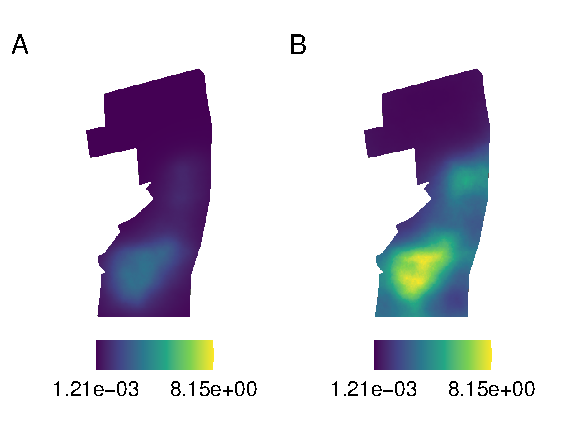
\includegraphics{figures/intensity_quantiles.pdf}
		\caption{Pointwise posterior quantiles for the intensity:  A) 0.025 quantile B) 0.975 quantile}
		\label{fig:intensity-quantiles}
	\end{center}
\end{figure}
These caveats make the map difficult to use for most non-statistically trained audiences and even trained statisticians may misinterpret these quantile maps.  To demonstrate the misleading nature of these maps, if we were to (incorrectly) treat the lower and upper quantile plots as though they were intensity surfaces and integrate them, then we would obtain an abundance estimate of approximately 2,900 for the 0.025 quantile map and 10,700 for the 0.975 quantile map.  However, these abundance estimates are not supported by the posterior for abundance (\autoref{fig:realized-abundance-posterior}).  In other words, these maps tempt an interpretation that is inconsistent with the very model that produced the maps.

Broadly speaking, we advocate for moving beyond maps of uncertainty presented for their own sake and towards model outputs that directly relate to the wider objectives of the analysis. We conclude that, although all useful in their own way, each of the mapped summaries of the posterior intensity field suffer from some weaknesses, whether through masking certain properties of the random field or through being difficult to interpret. In the following section we suggest an approach that avoids some, but not all, of the pitfalls above.

\subsection{Identification of hotspots}

In this section we consider the hypothetical challenge of using our model to identify population hotspots within Hakalau refuge.  This acts as a focus for communication that directs our choices when producing model outputs.

A solution to the problem of interpreting quantile and exceedance probability maps is to use methods that explicitly consider the joint probability of events across all prediction locations. One option is to use excursions sets and excursion functions \citep{bolin_excursion_2015}.  This requires users to choose thresholds of interest (e.g. the definition of a hotspot), and to select an acceptable level of uncertainty in knowing whether the field exceeds this threshold.  This forces us to consider this explicitly and leaves us less at the whim of an arbitrary colour scale.  Crucially, excursion sets and functions can be estimated using Monte Carlo samples and so fit well within our one-stage Bayesian approach.

We provide the technical definition of excursion sets and functions below, using the same notation as \cite{bolin_excursion_2015}.  For readers unfamiliar with these methods, the notation can take some getting used to.  However, the precise mathematical definitions are useful when it comes to interpreting these methods.  We try to, as much as possible, give an informal explanation alongside the mathematical description.  The positive excursion set with level $u$ for a deterministic function $f(\bs)$ with domain $\Omega$ is $A_u^{+}(f) = \{ \bs \in \Omega ; f(\bs) > u \}$, i.e. the set of all locations in $\Omega$ where $f$ exceeds a threshold value $u$. For a random field, $\lambda(\bs)$, the positive excursion set with level $u$ and probability $1 - \alpha$ is
\begin{equation*}
E_{u,\alpha}^{+}(\lambda) = \argmax_{D}\{\lvert D \rvert : \mathbb{P}\left[D \subset A_u^{+}(\lambda)\right] \geq 1 - \alpha \} .
\end{equation*}
In other words, the positive excursion set $E_{u,\alpha}^{+}(\lambda)$ is the \textit{largest} set of locations for which realisations of $\lambda(\bs)$ exceed the threshold $u$, \textit{simultaneously}, for all locations in the set, with probability $1-\alpha$.  Note that we must decide on relevant choices for $u$ and $\alpha$ given the aims and context of the analysis.  Negative excursion sets are similarly defined.  Excursion sets can be estimated by considering candidate sets for $D$ of increasing size and a sequential integration scheme to estimate the required probabilities in a computationally efficient way.  A full description of the methods is given in \cite{bolin_excursion_2015} and a software implementation in the \texttt{excursions} package \citep{bolin_calculating_2018}.  

\autoref{fig:excursions}A shows the positive excursion set with a level corresponding to 1 bird per hectare with probability 0.95 (hence $\alpha = 0.05$).  Note that we use this threshold as the definition of a hotspot, and proceed with generating model results that incorporate this definition.  This figure can be interpreted in a natural way as the largest region for which the intensity is greater than 1 bird per hectare for every location within the region, with probability 0.95. 
\begin{figure}[!htb]
	\includegraphics{figures/excursions.pdf}
	\caption{A) The blue area is the positive excursion set with a level corresponding to 1 bird per hectare and probability 0.95.  B) The positive excursion function with a level corresponding to 1 bird per hectare.  The scale shows the probability values $1-\alpha$.}
	\label{fig:excursions}
\end{figure} 
This map could be used to define, for example, a `core region' for the \akepa{} population, with particular conservation importance.  Crucially, this map depends on a clear mathematical description of what a `core region' actually means in a statistical sense.  While any particular definition would be up for debate, the advantage is that the statistical methodology is taken as close as possible to the aims of the analysis.  Often a map of species density will be interpreted informally in many different ways (one of which is identifying hotspots).  To visualise how such excursion sets change with different levels of uncertainty we can use the excursion function $F_u^{+}(\bs) = \sup \{1 - \alpha ; \bs \in E_{u,\alpha}^+ \}$.  This defines, for each location, the largest possible probability $1 -\alpha$ for which that location would be in the excursion set defined using probability $1 - \alpha$.  That is, if we allow greater uncertainty, this function shows which locations would be included in the excursion set.    

The excursion function with a level corresponding to 1 bird per hectare is shown in \autoref{fig:excursions}B.  It is clear from the figure that regions close to the edge of the excursion set with $\alpha = 0.05$ would be included if the $\alpha$ value were allowed to increase slightly.  Similarly, the core of the high density region seems to exceed 1 bird per hectare even for $\alpha$ levels close to zero. This map could be used to identify, for example, secondary areas of potential importance beyond the core population that could be investigated further.

\section{Discussion}
\label{sec-discussion}

There are several natural extensions to the model presented here.  Spatio-temporal models can also be fitted using \texttt{R-INLA}, which would allow multiple years of data to be modelled jointly, as was the case in \cite{camp_dsm_2020}.  Another extension is to develop the observation process model by considering other detection functions or including covariates, for example.  Factors such as weather conditions, observer expertise, animal behaviour and morphological traits are likely to affect detectability.

The iterated INLA inference procedure has the potential to be applied to other non-linear model components that arise in spatial statistics.  We note two promising areas within the field of spatial ecology that highlight this potential: 

\begin{itemize}
	\item \textbf{Selectivity analysis} In surveys of the marine environment, the size, length and weight of fish affects the likelihood of being caught in a trawl net.  The probability of capture is typically modelled as a logistic function with parameters that depend on morphological traits \citep{herrmann_understanding_2016, madsen_selectivity_2007, galbraith_demersal_1994}.  This function is analogous to the detection function in distance sampling models.  Our framework allows for the joint modelling of selectivity and spatial data.
	\item \textbf{Functional responses} The concept of a `functional response' captures the idea that the overall abundance of a resource or risk will affect a species' response to it \citep{holling_some_1959}.  These varying responses can be described mathematically using parametric equations that have the desired properties, e.g. an increasing function with a horizontal asymptote, to capture the notion of diminishing returns.  Such non-linear functions could be incorporated within our framework
\end{itemize}

The popularity of using INLA for spatial modelling has grown, in large part, due to the computational efficiency of the approach.  However, this efficiency comes at the cost of reduced flexibility in model specification over, say, a more general probabilistic programming language such as \texttt{JAGS} \citep{plummer_jags_2017} or \texttt{Stan} \citep{stan_Rstan_2020}.  The iterated INLA approach allows a wider class of models to be considered whilst retaining much of the computational benefits of INLA.  In addition to computational efficiency, there are some features of INLA that are not generally available in other packages, such as: (i) the ability to model using GRFs directly on the sphere, avoiding projecting to $\mathbb{R}^2$ \citep{lindgren_explicit_2011}; (ii) GRFs that account for complex barriers such as coastlines and islands, to avoid inappropriately smoothing across these \citep{bakka_NonstationaryGaussianModels_2019}; and (iii) support for joint likelihood models, allowing modelling of, for example, marked point processes \citep{illian_FittingComplexEcological_2013}, and combining multiple data sources.  These approaches can now readily be incorporated into distance sampling analyses, as well as broader spatial ecology and spatial statistics applications. 

\section*{Data Availability} 

Hawaii Akepa (Loxops coccineus) point transect distance sampling data were provided by U.S. Fish and Wildlife Service, Hakalau Forest Unit of the Big Island National Wildlife Refuge Complex. The 2002 survey data are available from the U.S. Geological Survey: \url{https://doi.org/10.5066/P9Q9UXMZ} \citep{camp_datarelease_2002}.  The data for 1987-2017 are also available  available from the U.S. Geological Survey: \url{https://doi.org/10.5066/P98IO297} \citep{camp_datarelease_all}. Code to reproduce the figures and results in this paper are available in a git repository and can be accessed at \url{https://github.com/ASeatonSpatial/point-transects-paper/}.

\section*{Acknowledgements}

We are grateful to the many U.S. Fish and Wildlife Service staff and volunteers who helped collect the data through the \hawaii Forest Bird survey. We thank Steve Buckland for helpful comments on an early draft.  We also thank Dave Miller for helpful discussions on density surface models and how they relate to point process models.  Any use of trade, firm, or product names is for descriptive purposes only and does not imply endorsement by the U.S. Government.

\clearpage
\bibliographystyle{rss}
\bibliography{paper}

\end{document}
